
\section{Results}
This section presents the results for PBE, CTS and KWS separately.
Afterwards we compare the three techniques with each other and RLR as
baseline.

\lstset{
  language=,
  morekeywords={Test, Output, Desired},
	basicstyle=\ttfamily\scriptsize,
  postbreak=\mbox{\textcolor{cyan}{$\hookrightarrow$}\space},
  showspaces=false,
  showstringspaces=false,
  keywordstyle=\textbf,
	frame=single,
  extendedchars=false,
  texcl=false
}
\begin{figure}[!t]
  \centering
  \begin{lstlisting}[breaklines=true]
Test Output:
Error: Invalid CSS after "2.3em": expected expression (e.g. 1px, bold), was ";"
        on line 86 of sass/components/dropdown.sass   
Desired Test Output:
Error: Invalid CSS after "2.3em": expected expression (e.g. 1px, bold), was ";"
        on line 86 of sass/components/dropdown.sass
        from line 5 of sass/components/_all.sass
        from line 6 of bulma.sass
  \end{lstlisting}  
  \caption{Example for an unsuccessful retrieval (PBE retrieved only two of the four targeted lines).}
  \label{lst:pbe-unsuccessful}
\end{figure}

\subsection{Common Text Similarity (CTS)}
\label{sec:r:cts}
\begin{figure*}
\centering
    \textbf{Common Text Similarity (CTS)}\par\medskip
\begin{subfigure}[t]{\columnwidth}
		\centering
                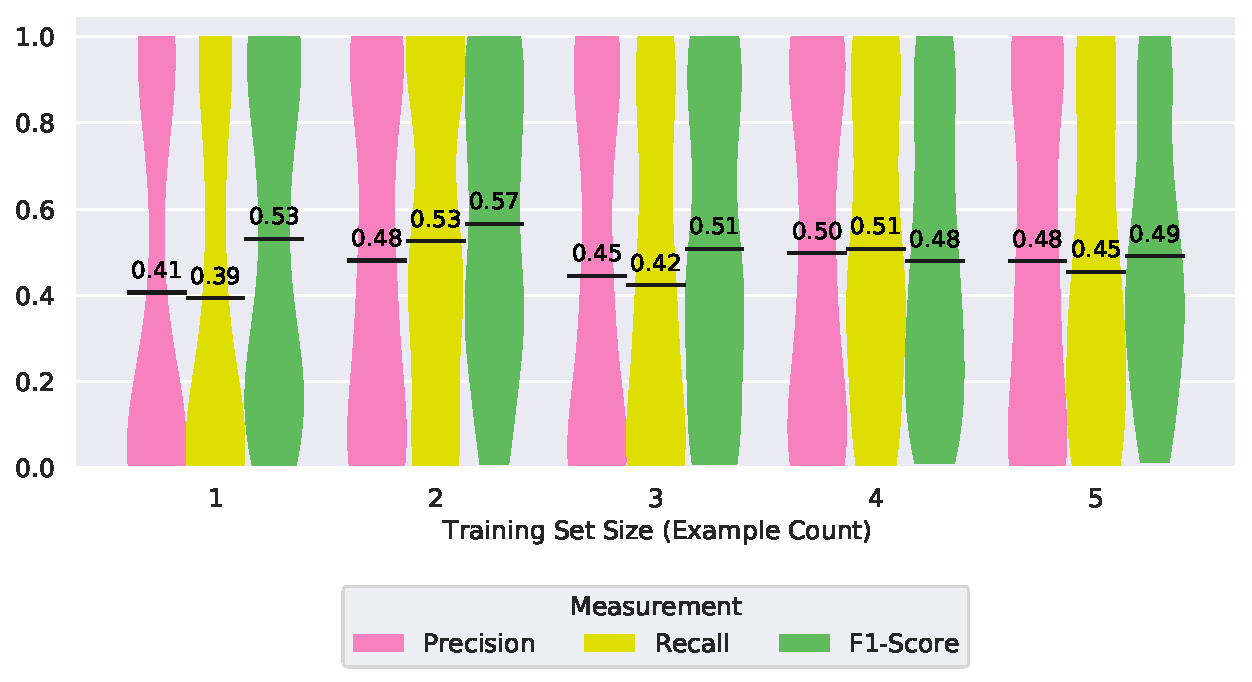
\includegraphics[width=\columnwidth, clip]{img/big-study/recall-precision-examplecount-CTS.pdf}
		\caption{Precision, recall and F$_{1}$-score for an increasing training set size.}
		\label{fig:recall-precision-examplecount-CTS}
                
\end{subfigure}\hspace{\fill}
\begin{subfigure}[t]{\columnwidth}
		\centering
                		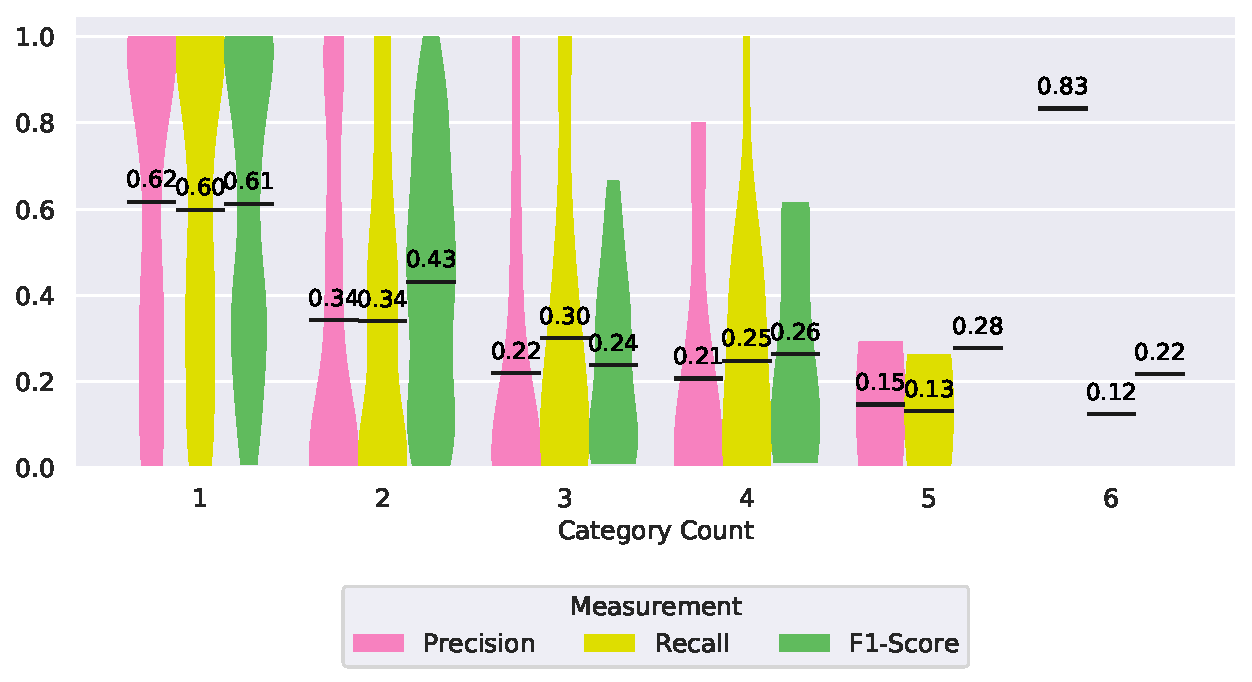
\includegraphics[width=\columnwidth, clip]{img/big-study/recall-precision-categorycount-CTS.pdf}
		\caption{Precision, recall and F$_{1}$-score for an increasing number of structural categories in the training and test sets.}
		\label{fig:recall-precision-categorycount-CTS}
\end{subfigure}
\caption{Results of chunk retrieval with Common Text Similarity (CTS)}
\end{figure*}

\Cref{fig:recall-precision-examplecount-CTS} presents precision,
recall and F$_{1}$-score of chunk retrieval using CTS for an
increasing number of training examples. When using one to five
training examples, the size of the training set has no noticeable
influence on precision, recall or F$_{1}$-score of the chunk retrieval
with CTS.

\Cref{fig:recall-precision-categorycount-CTS} shows the same
measurements for an increasing number of structural categories in the
training and test examples. With increasing category count, precision,
recall and F$_{1}$-score decrease. Especially for more than three
categories present we have no chunk retrieval runs where all desired
lines were extracted.

\subsection{Keyword Search (KWS)}
\label{sec:r:kws}
\begin{figure*}
\centering
    \textbf{Keyword Search (KWS)}\par\medskip
\begin{subfigure}[b]{\columnwidth}
		\centering
		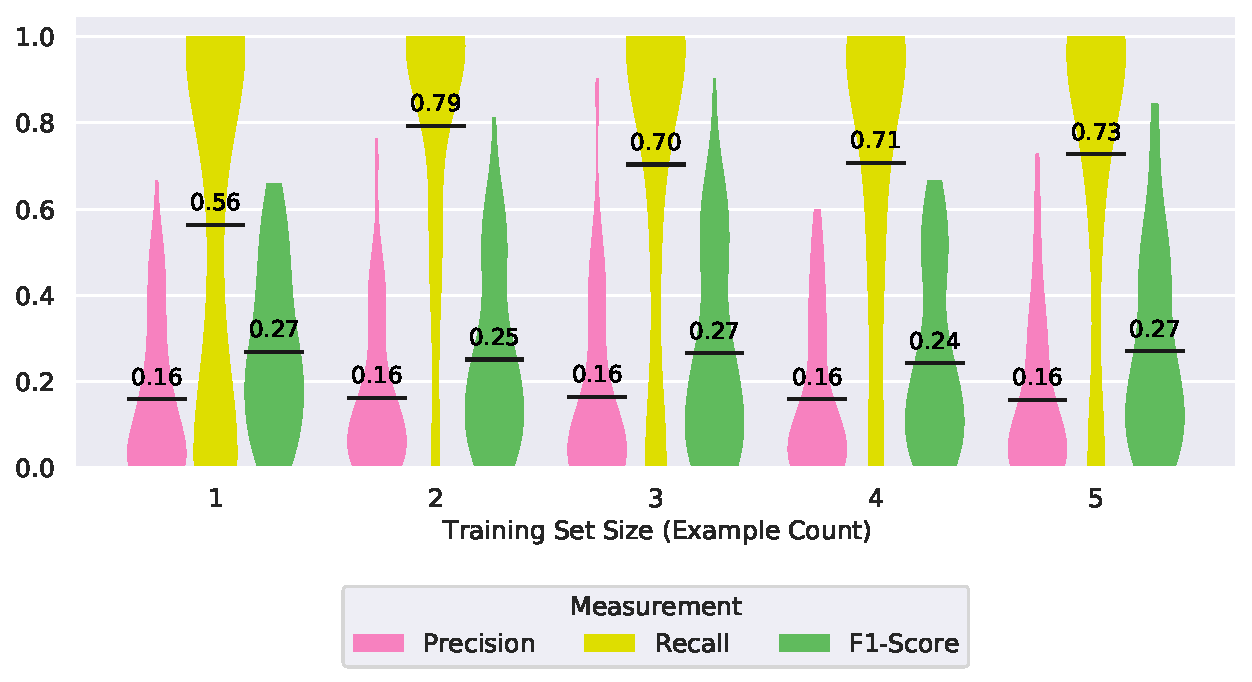
\includegraphics[width=\columnwidth, clip]{img/big-study/recall-precision-examplecount-KWS.pdf}
		\caption{Precision, recall and F$_{1}$-score for an increasing training set size.}
		\label{fig:recall-precision-examplecount-KWS}
\end{subfigure}\hspace{\fill}
\begin{subfigure}[b]{\columnwidth}
		\centering
		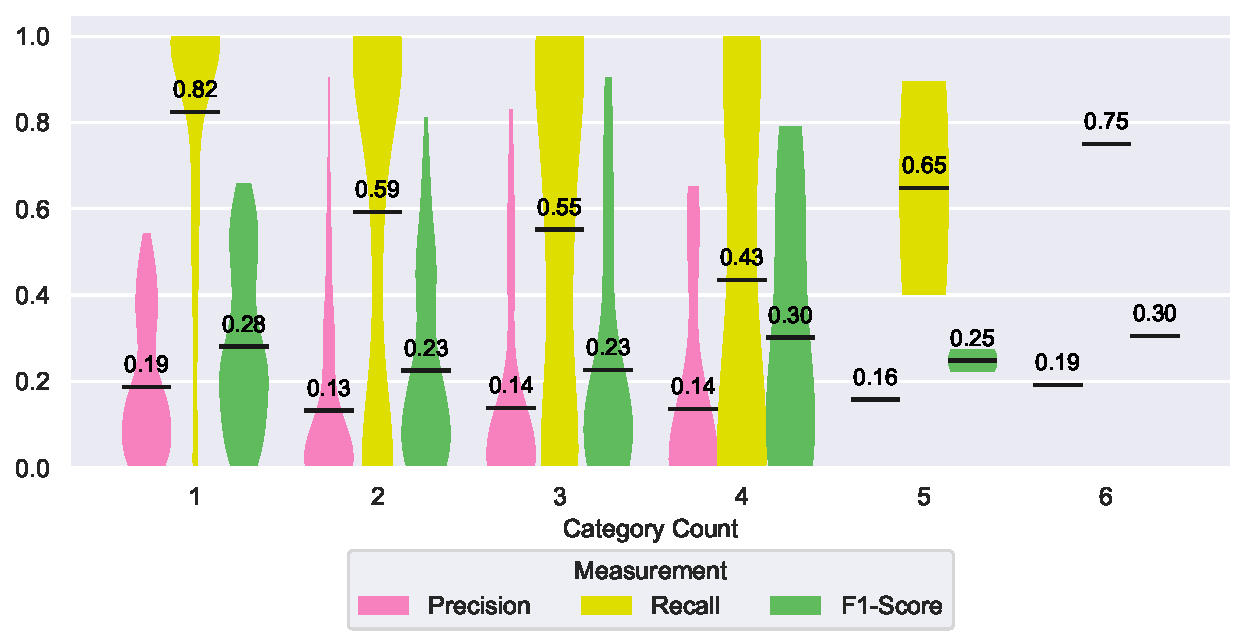
\includegraphics[width=\columnwidth, clip]{img/big-study/recall-precision-categorycount-KWS.pdf}
		\caption{Precision, recall and F$_{1}$-score for an increasing number of structural categories in the training and test sets.}
		\label{fig:recall-precision-categorycount-KWS}
\end{subfigure}
\caption{Results of chunk retrieval with Keyword Search (KWS)}
\end{figure*}


\Cref{fig:recall-precision-examplecount-KWS} presents precision,
recall and F$_{1}$-score of chunk retrieval using KWS for different
numbers of training examples. The recall increases by about 12\% when
increasing the size of the training set to more than one example,
while the precision stays constant at around 16\%. The F$_{1}$-score
stays around 26\%.

\Cref{fig:recall-precision-categorycount-KWS} shows the same
measurements for an increasing number of structural categories in the
training and test examples. For more than one structural category in
the training and test examples the recall decreases by about 20\% and
the precision decreases about 6\%. For more than two structural
categories no clear trend is visible in precision, recall or
F$_{1}$-score for an increasing amount of categories in the training
and test examples.

% Figure~\ref{fig:contextsizefactor-precision-recall-KWS} shows the
% effect of the retrieval size factor on precision, recall and
% F$_{1}$-score of chunk retrieval runs with KWS\@. The precision is
% 19\% when retrieving half of the expected number of lines. On
% average 9\% of the lines in the build log are retrieved then. When
% 2.5 times the expected number of lines are retrieved, the precision
% decreases to 10\% and a quarter of the lines in the build log are
% retrieved on average. The recall ranges from 58\% to 75\% and the
% F$_{1}$-score shows a constant decrease from 29\% to 17\%.

% \begin{figure}[!t]
% 		\centering
% 		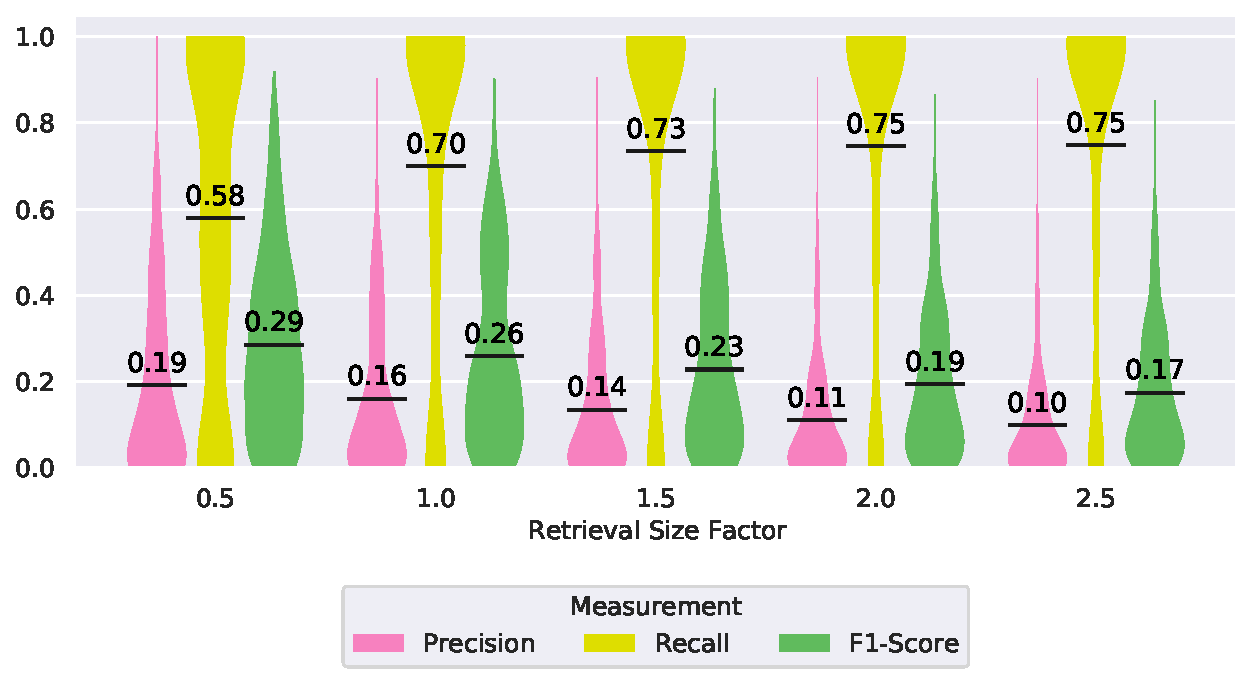
\includegraphics[width=\columnwidth, clip]{img/big-study/contextsizefactor-precision-recall-KWS.pdf}
% 		\caption{Precision, recall and F$_{1}$-score of chunk retrieval with KWS compared to retrieval size factor.}
% 		\label{fig:contextsizefactor-precision-recall-KWS}
% \end{figure}

\subsection{Program Synthesis by Example (PBE)}
\label{sec:r:pbe}
\begin{figure*}
\centering
    \textbf{Program Synthesis by Example (PBE)}\par\medskip
\begin{subfigure}[b]{\columnwidth}
		\centering
		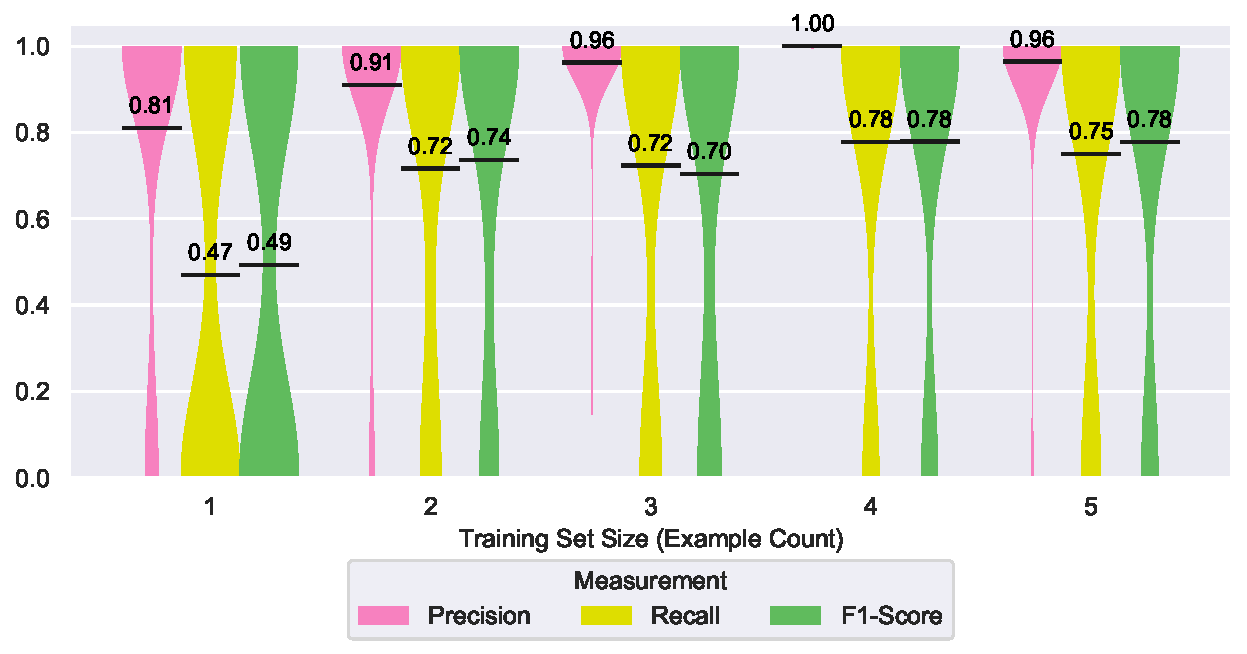
\includegraphics[width=\columnwidth, clip]{img/big-study/recall-precision-examplecount-sythesisworked-PBE.pdf}
                		\caption{Precision, recall and F$_{1}$-score when PBE could synthesize a consistent program compared with the size of the training set.}
                \label{fig:recall-precision-examplecount-sythesisworked-PBE}
\end{subfigure}\hspace{\fill}
\begin{subfigure}[b]{\columnwidth}
		\centering
		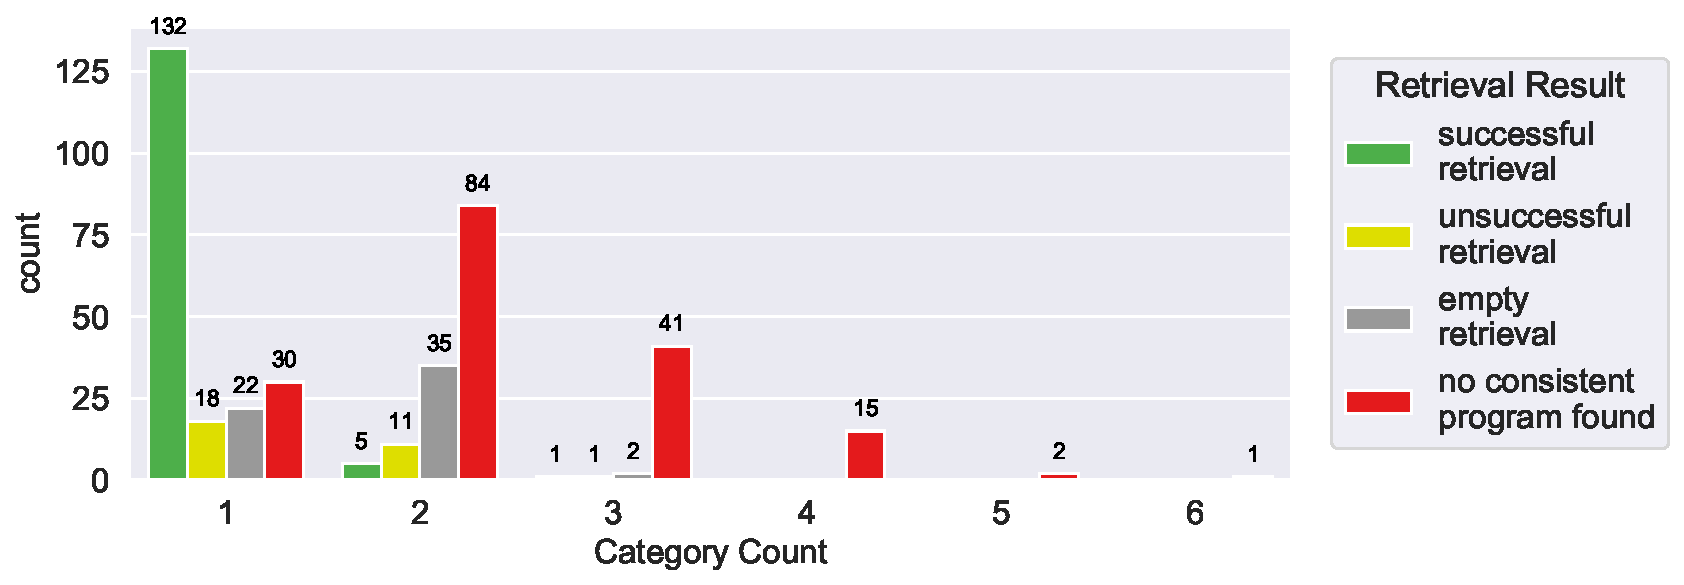
\includegraphics[width=\columnwidth, clip]{img/big-study/failure-reason-categorycount-PBE.pdf}
                		\caption{Increasing number of structural categories in the training and test sets.}
                \label{fig:failure-reason-categorycount-PBE}
\end{subfigure}
\caption{Results of chunk retrieval with  Program Synthesis by Example (PBE)}
\end{figure*}


\begin{figure}[tbp]
		\centering
		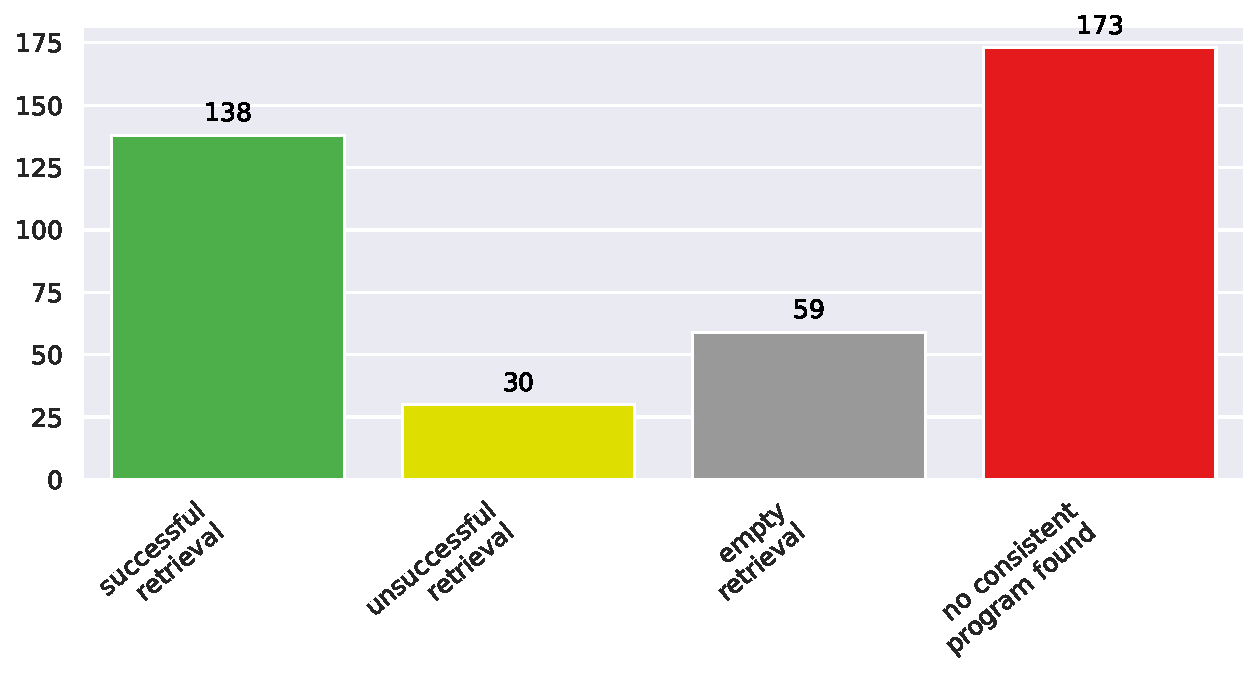
\includegraphics[width=0.75\columnwidth, clip]{img/big-study/failure-reason-pbe.pdf}
		\caption{Results of chunk retrieval with PBE.}
		\label{fig:failure-reason-PBE}
\end{figure}

\Cref{fig:failure-reason-PBE} shows the results of the PBE runs in our
evaluation. Out of the 400 runs, 5 per each one of the 80 example
sets, PBE extracted all the desired lines in 138 cases. In 89 further
cases, an extraction program was also successfully synthesized, though
in 59 of the 89 cases the synthesized program yielded no output. In 30
of the 89 cases did the synthesized program only partially extract a
subset of the desired lines. For these 30 cases, the average recall
was 28\%. Listing \ref{lst:pbe-unsuccessful} shows an example of such
an \emph{unsuccessful retrieval}, where the synthesized program only
retrieved two of the four targeted lines. In 173 of the 400 cases
could PROSE not synthesize program consistent with all of the training
examples.

\Cref{fig:failure-reason-categorycount-PBE} shows the results of PBE
runs depend on the number of structural categories in the training and
test examples. The figure demonstrates that program synthesis mostly
returns exactly the desired output when there are is only one
structural category present in the training examples. However, when
two or more structural categories are simultaneously present in the
examlpe set, PROSE could in most cases not synthesize a program
consistent with all training examples. For four or more present
categories PROSE could never synthesize a consistent program.

\Cref{fig:recall-precision-examplecount-sythesisworked-PBE} shows
precision and recall of the 227 runs where PBE could synthesize a
program consistent with all training examples. When the training set
size increases from one to two, recall and F$_{1}$-score increase by
about 25\%, precision increases by about 10\%. For two or more
training examples, recall and F$_{1}$-score stay around 75\% and
precision around 96\%.

\subsection{Random Line Retrieval}
\label{sec:r:rlr}

In our evaluation, we compare against a baseline of randomly
picking lines from the build log. Its results follow intuitive
expectations:
The precision ranges between 8\% and 5\%, the recall between 6\% and
8\%. The size of the training set has no visible impact on either.
An greater number of structural categories within the training and
test sets decreased the precision of RLR from 7\% to 0\%, the recall
increases from 6\%, for one structural category present, to 11\%, for
three sturctural categories present and also drops to 0\% for more
structural categories.
Graphs of the results of the chunk retrieval with RLR from our study
are included in our replication package~\cite{brandt2020chunk-replication}. 

\subsection{Comparison of All Techniques}
In this section, we aggregate the results from
\Cref{sec:r:kws,sec:r:pbe,sec:r:cts,sec:r:rlr} and put them next to it
each other.

\Cref{fig:success-partial-all} compares the success of chunk
retrievals differentiated by techniques in our study. CTS and KWS
extract some of the desired lines in 79\% and 88.5\% of the chunk
retrieval runs. With 38.25\%, KWS also has the highest number of fully
successful extractions, followed by PBE with 34.5\%. PBE has the
lowest number of partial retrievals with only 18 out of 400 chunk
retrieval runs.

% The averaged precision, recall and F$_{1}$-score f all techniques is
% compared in Figure~\ref{fig:recall-precision-all}. The recall of PBE
% has a high skew towards one and zero, meaning in most cases either
% the retrieval is successful or no relevant lines are extracted at
% all. PBE has the highest average precision with 95\%. Chunk
% retrieval with CTS has the highest average F$_{1}$-score with 51\%
% and the second highest recall with 46\%. KWS has the smallest
% precision of the three chunk retrieval techniques. With 16\% it is
% still higher than the precision of the RLR baseline with 7\%. KWS
% has the highest recall of all techniques with 70\%.

\Cref{fig:recall-precision-singlecategory-all,fig:recall-precision-multicategory-all}
show the influence of a single structural category present in the
training examples compared to multiple categories present. For more
than one category being present, the recall of PBE decreases greatly.
For CTS and KWS the values also decrease, while RLR is not affected by
the number of structural categories present.

\begin{figure}[!t]
		\centering
		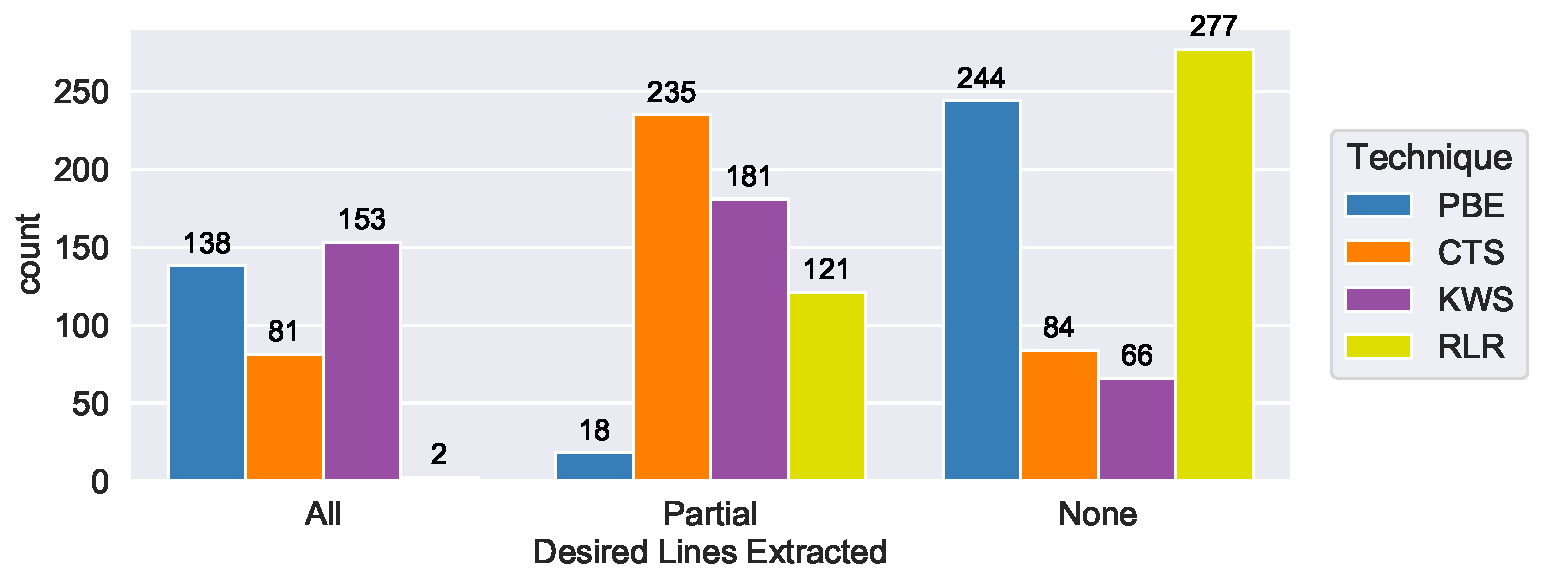
\includegraphics[width=\columnwidth, clip]{img/big-study/success-partial-all.pdf}
		\caption{Success of chunk retrievals for all techniques.}
		\label{fig:success-partial-all}
\end{figure}

\begin{figure*}
\centering
    \textbf{PBE, CTS, KWS, and RLR}\par\medskip
\begin{subfigure}[b]{\columnwidth}
		\centering
                		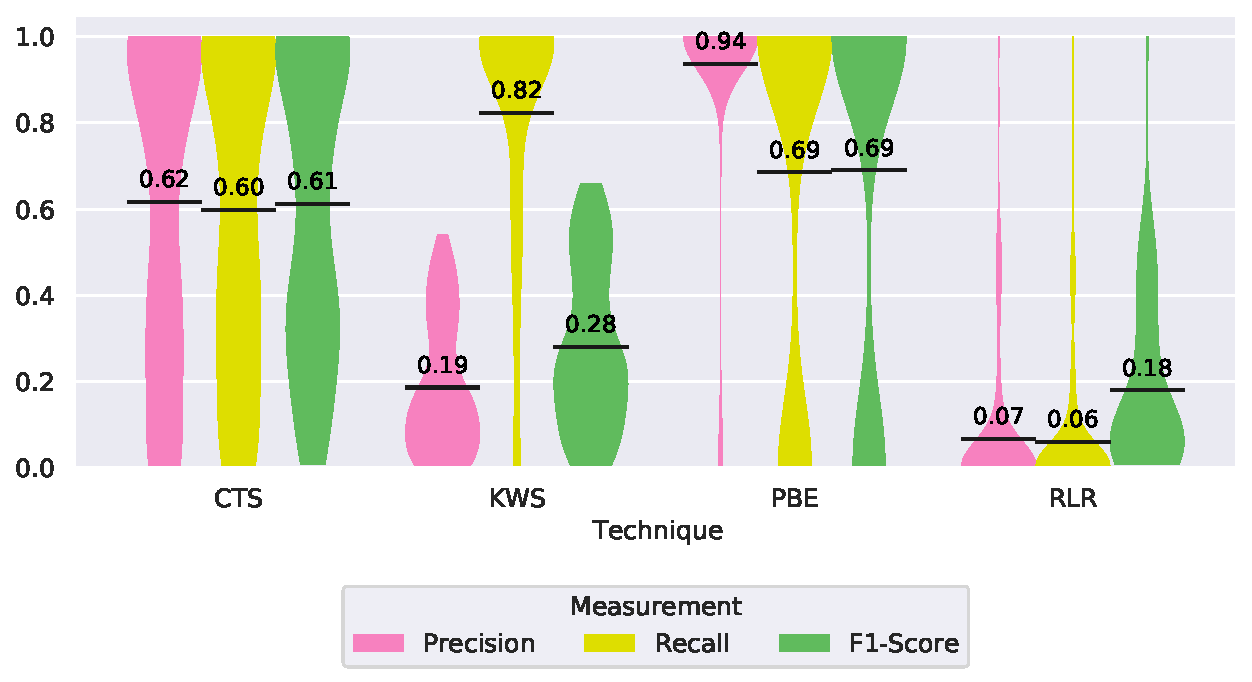
\includegraphics[width=\columnwidth, clip]{img/big-study/recall-precision-singlecategory-all.pdf}
		\caption{Precision, recall and F$_{1}$-score of all techniques when training examples are in \emph{one} structural category.}
		\label{fig:recall-precision-singlecategory-all}
\end{subfigure}\hspace{\fill}
\begin{subfigure}[b]{\columnwidth}
		\centering
                		\centering
		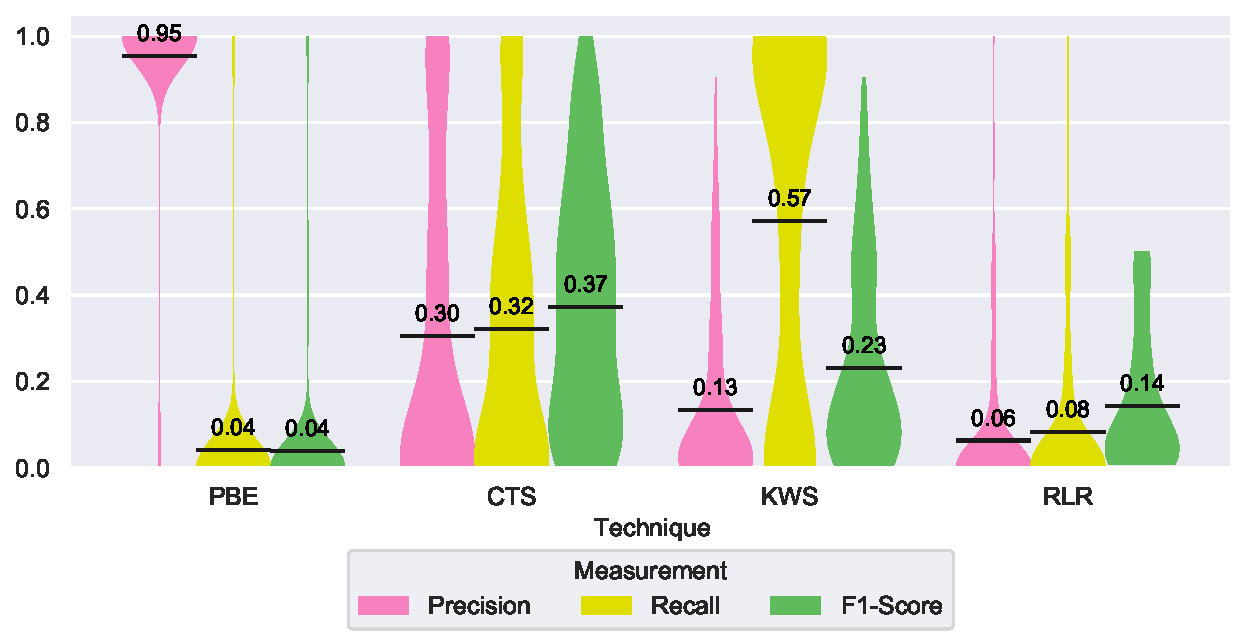
\includegraphics[width=\columnwidth, clip]{img/big-study/recall-precision-multicategory-all.pdf}
		\caption{Precision, recall and F$_{1}$-score of all techniques when training examples are in \emph{more than one} structural categories.}
		\label{fig:recall-precision-multicategory-all}
\end{subfigure}
\caption{Comparison of all chunk retrieval techniques, split by structural category count.}
\end{figure*}
